\documentclass[14pt, openany]{article}
\usepackage[utf8]{inputenc}
\usepackage[T1]{fontenc}
\usepackage{hyperref}
\usepackage[french]{babel}
\frenchbsetup{StandardLists=true}
\usepackage{amsmath,amsfonts,amssymb}
\usepackage{graphicx}
\usepackage[a4paper,left=2cm,right=2cm,top=2cm,bottom=2cm]{geometry}
\usepackage{bbm}
\usepackage{libertine}
\usepackage{color}
\usepackage{array,multirow,makecell}
\usepackage{enumitem} %Pour modifier les puces
\usepackage{caption}
\usepackage{dsfont}
\newcolumntype{R}[1]{>{\raggedleft\arraybackslash }b{#1}}
\newcolumntype{L}[1]{>{\raggedright\arraybackslash }b{#1}}
\newcolumntype{C}[1]{>{\centering\arraybackslash }b{#1}}
\setlength{\parindent}{0cm}
\setlength{\parskip}{1ex plus 0.5ex minus 0.2ex}
\newcommand{\hsp}{\hspace{20pt}}
\newcommand{\HRule}{\rule{\linewidth}{0.5mm}}
\AddThinSpaceBeforeFootnotes
\FrenchFootnotes

%%%% debut macro %%%%
\newenvironment{changemargin}[2]{\begin{list}{}{%
\setlength{\topsep}{0pt}%
\setlength{\leftmargin}{0pt}%
\setlength{\rightmargin}{0pt}%
\setlength{\listparindent}{\parindent}%
\setlength{\itemindent}{\parindent}%
\setlength{\parsep}{0pt plus 1pt}%
\addtolength{\leftmargin}{#1}%
\addtolength{\rightmargin}{#2}%
}\item }{\end{list}}
%%%% fin macro %%%%

\begin{document}

\begin{titlepage}
\begin{center}
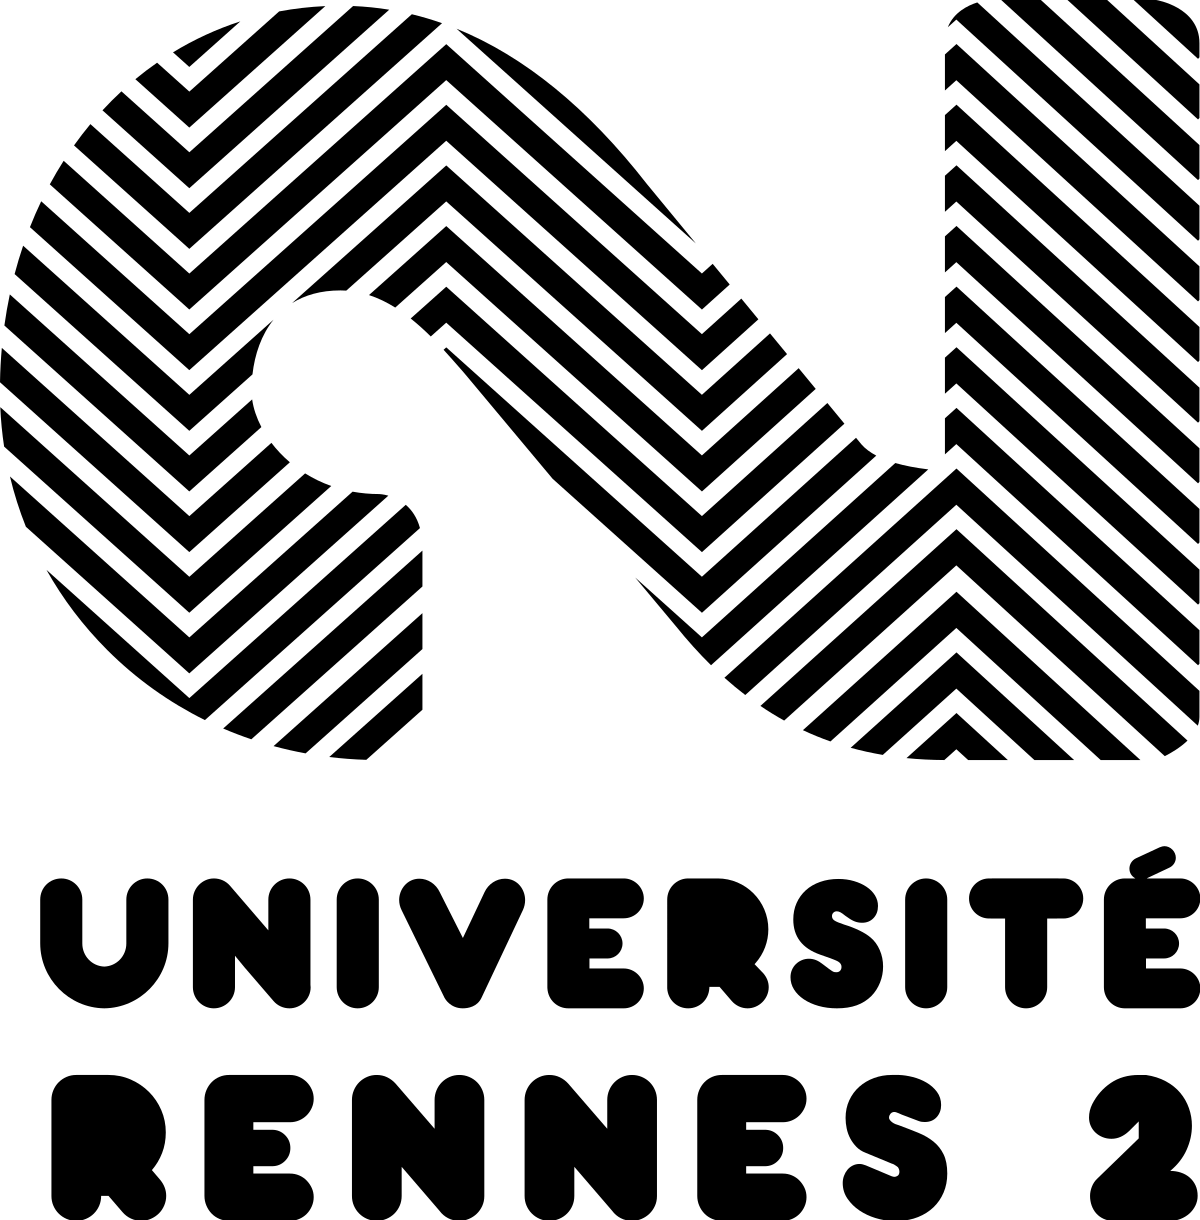
\includegraphics[scale=0.15]{Images/ur2.png}\\
\bigskip
\textsc{\Large PROJET DATA SCIENCE - MASTER 2 MAS PARCOURS SCIENCES DES DONNEES\\ 
\bigskip
Rapport de l'étude}\\
\bigskip
    \HRule \\[0.4cm]
    { \huge \bfseries Prédictions des températures de 7 stations différentes à un horizon de 36 heures\\[0.4cm] }
        \HRule \\[2cm]
   \begin{figure}[h]
    \begin{minipage}[c]{.46\linewidth}
        \centering
        
\includegraphics[scale=0.3]{Images/defi.png}
    \end{minipage}
    \hfill%
    \begin{minipage}[c]{.46\linewidth}
        \centering
        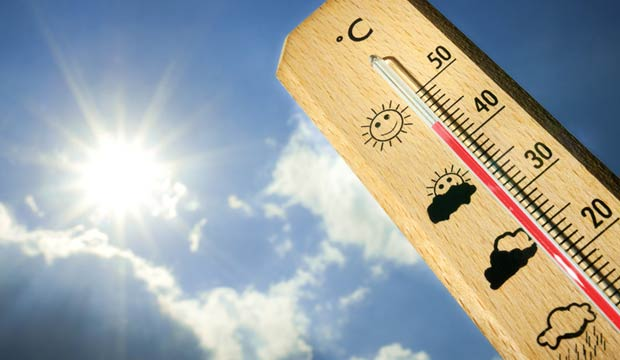
\includegraphics[scale=0.36]{Images/temp.jpg}
    \end{minipage}
	\end{figure}
    \bigskip
    \begin{minipage}{0.4\textwidth}
      \begin{flushleft} \large
      \emph{Team :} \textsc{Freak-unit}\\
      \emph{Membres :}
      \begin{itemize}
      	\item \textsc{Benjamin ALLEAU}\\
      	\item \textsc{Abdessamad AZNAGUE}\\
        \item \textsc{Guillaume LE FLOCH}\\
      \end{itemize}
      \end{flushleft}
    \end{minipage}
    \begin{minipage}{0.4\textwidth}
      \begin{flushright} \large
      	\emph{Organisateur :} \textsc{INSA de Toulouse}
        \emph{Encadrant :} \textsc{M. Romain TAVENARD}\\         
      \end{flushright}
    \end{minipage}

    \vfill
    
    % Bottom of the page
    {\large 05 Octobre 2017 —  08 Janvier 2018}

\end{center}
\end{titlepage}

\renewcommand{\contentsname}{Plan}

\tableofcontents
\newpage

\section{Présentation du projet}
\paragraph{}
La compétition 2017-2018 est basée sur une stratégie d'adaptation statistique pour améliorer la prévision de températures à un horizon de 36 heures.

Les services du \textbf{CNRM} (Centre National de Recherches Météorologiques) construisent des grands modèles déterministes de l'atmosphère par résolution des équations de Navier et Stockes sur un maillage: 10km pour \textbf{ARPEGE}, kilométrique pour \textbf{AROME} mais limité à l'Europe. Il apparaît que ces modèles sont généralement biaisés, notamment parce qu'ils ne peuvent prendre en compte des phénomènes à petite échelle. Par exemple, un vent important (e.g. vent d'autan à Toulouse) provoque des turbulences qui, en mélangeant les couches d'air, entrainent une baisse de la température par rapport à celle prévue.

Un modèle statistique intégrant les prévisions du modèle déterministe peut contribuer à réduire significativement ces biais. En revanche, un modèle statistique seul est incapable de prévoir l'arrivée d'une perturbation océanique à partir de données locales. L'adaptation statistique est donc une mise en collaboration \og optimale \fg{} des deux approches de modélisation, déterministe et statistique.

Le \og Défi Grosses Data \fg{} est donc un challenge mettant en confrontation une multitude de groupes d'étudiants provenant des \textbf{INSA} de Toulouse et Rennes, ainsi que des Universités de \textbf{Bordeaux}, \textbf{Rennes 1}, \textbf{Rennes 2}, \textbf{Paris Descartes}, \textbf{Paul Sabatier (Toulouse 3)} ou encore la \textbf{Toulouse School of Economics}. Ce rapport détaillera le travail fourni par l'équipe \textbf{Freak-unit}, une des 8 équipes représentant l'\textbf{Université de Rennes 2}.

L'objectif de ce projet est simple : prédire au mieux les températures de 7 stations sur un horizon de 36 heures. Pour ce faire, 36 fichiers $train\_H.csv$ $(H=1,..,36)$, ont été mis à notre disposition. Ces fichiers contiennent les variables issues des modèles physiques décrits dans le préambule à un horizon de +H heures. Leur contenu est le suivant :
\begin{itemize}
\item les lignes correspondent à chaque jour sur une période allant du $1^{er}$ janvier 2014 au 30 mai 2016.
\item les colonnes contiennent 30 variables (température, nébulosité, vent, humidité ..)
\end{itemize}
Nous allons détailler ces variables afin de bien comprendre quelles sont les mesures à notre disposition :
\begin{itemize}
\item \textbf{insee} : Facteur à 7 niveaux représentant le numéro insee des stations pour lesquelles nous cherchons à prédire les températures (Nice, Toulouse Blagnac, Bordeaux-Mérignac, Rennes, Lille Lesquin, Strasbourg Entzheim, Paris-Montsouris)
\item \textbf{tH2\_obs} : Observation de la température à 2 mètres \textit{in situ} au point station (prédictant). \textbf{C'est la variable réponse que l'on cherche à prédire}
\item \textbf{ech} : Facteur à 36 niveaux correspondant à l'échéance de validité (H)
\item \textbf{capeinsSOL0} : Energie potentielle convective
\item \textbf{ciwcH20} : Fraction de glace nuageuse à 20 mètres
\item \textbf{clwcH20} : Fraction d'eau nuageuse à 20 mètres
\item \textbf{nH20} : Fraction nuageuse à 20 mètres
\item \textbf{pMER0} : Pression au niveau de la mer
\item \textbf{rr1SOL0} : Précipitation horaire au niveau du sol
\item \textbf{rrH20} : Précipitation horaire à 20 mètres
\item \textbf{tpwHPA850} : Température potentielle au niveau 850 hPa
\item \textbf{ux1H10} : Rafale 1 minute du vent à 10 mètres composante zonale
\item \textbf{vapcSOL0} : Colonne de vapeur d'eau
\item \textbf{vx1H10} : Rafale 1 minute du vent à 10 mètres composante verticale
\item \textbf{ddH10\_rose4} : Facteur à 4 niveaux indiquant la direction du vent à 10 mètres (en rose4)
\item \textbf{ffH10} : Force du vent à 10 mètres en m/s
\item \textbf{flir1SOL0} : Flux Infra-rouge en J/$m^2$
\item \textbf{fllat1SOL0} : Flux de chaleur latente en J/$m^2$
\item \textbf{flsen1SOL0} : Flux de chaleur sensible en J/$m^2$
\item \textbf{flvis1SOL0} : Flux visible en J/$m^2$
\item \textbf{hcoulimSOL0} : Hauteur de la couche limite en mètres
\item \textbf{huH2} : Humidité 2mètres en \%
\item \textbf{iwcSOL0} : Réservoir neige kg/$m^2$ (équivalent en eau liquide des chutes de neige
\item \textbf{nbSOL0\_HMoy} : Nébulosité basse (moyenne sur les 6 points de grille autour de la station) (fraction en octat du ciel occulté)
\item \textbf{ntSOL0\_HMoy} : Nébulosité totale (moyenne sur les 6 points de grille autour de la station)
\item \textbf{tH2} : Température à 2 mètres du modèle \textbf{AROME}
\item \textbf{tH2\_VGrad\_2.100} : Gradient vertical de température entre 2 mètres et 100 mètres
\item \textbf{tH2\_XGrad} : Gradient zonal de température à 2 mètres
\item \textbf{tH2\_YGrad} : Gradient méridien de température à 2 mètres
\item \textbf{mois} : Facteur à 12 niveaux représentant le mois
\end{itemize}
Il est à noter que ces 36 fichiers \textit{train} contiennent des valeurs manquantes, le sujet sera approfondi un peu plus tard dans l'étude.

L'objectif de ce projet est le suivant : à partir des différents fichiers \textit{train} nous devons réaliser un apprentissage (supervisé dans notre cas) afin de pouvoir appliquer par la suite notre modèle au fichier \textit{test.csv} qui contient les mêmes variables, à l'exception de \textbf{tH2\_obs} évidemment puisqu'il faut la prédire. Les lignes du fichier \textit{test.csv} contiennent les 6 périodes de 15 jours suivantes :
\begin{itemize}
\item du 20/06/2016 au 02/07/2016
\item du 01/08/2016 au 14/08/2016
\item du 12/09/2016 au 25/09/2016
\item du 24/10/2016 au 06/11/2016
\item du 05/12/2016 au 18/12/2016
\item du 08/05/2017 au 21/05/2017
\end{itemize}
Une fois les prédictions effectuées, il faut soumettre les résultats sous forme d'un fichier au format \textit{csv} toujours, sur le site internet du challenge. Au bout d'exactement 1 heure après la soumission, nous pouvons visualiser notre score. La métrique utilisée pour évaluer le score est le \textbf{RMSE} (Root Mean Square Error). Si l'on note $\hat{y}$ notre vecteur de prédictions et $y_{obs}$ les valeurs des températures réellement observées, le \textbf{RMSE} associé se note :\\
\begin{center}
$RMSE_{\hat{y}} = \sqrt{\frac{1}{n} \sum\limits_{i=1}^n (\hat{y_i}-y_{obs_i})^2}$
\end{center}
En d'autres termes, cette métrique permet de mesurer d'une certaine façon l'écart entre nos prédictions et la réalité. Il est à noter que le challenge fournit un score de $1.30755$ appelé \textbf{Baseline} qui correspond à un score de référence, associé à \og un modèle élémentaire de prévision sans effort particulier d'optimisation. C'est un objectif a minima à améliorer dans ce concours \fg{}. Le décor est planté, désormais il ne reste plus qu'à se lancer dans le challenge.
\section{Remerciements}
\paragraph{}
Avant de détailler les différentes étapes de ce projet, les 3 membres de la \textbf{Freak-unit} team souhaitent remercier tout particulièrement leur professeur encadrant, \textbf{M. Romain TAVENARD} pour son accompagnement tout au long du projet et pour l'aide apportée. Sa connaissance du \textit{Deep Learning} aura notamment été un facteur déterminant dans la réussite de ce projet.

\section{Différentes stratégies envisagées}
\paragraph{}
Afin d'effectuer l'analyse la plus fine et pertinente possible, il est primordial de bien définir la stratégie d'étude à adopter. Par \og stratégie \fg{}, nous parlons ici de la façon dont nous allons structurer les données, des techniques que nous allons employer pour optimiser la performance des algorithmes. Cela peut être vu comme un problème d'optimisation sous contrainte : notre objectif est de réaliser la meilleure performance sous des contraintes de temps et de matériel. Il faut donc réussir à combiner au mieux la théorie mathématique avec la réalisation informatique.

\subsection{Structuration des données}
\paragraph{}
Un premier travail a consisté à agréger les données des 36 fichiers $train\_H.csv$ $(H=1,..,36)$ dans un seul jeu de données : cela aboutit à une matrice de $189 281$ lignes et $31$ colonnes. Dans un deuxième temps, nous avons divisé ce fichier en $7$ sous-fichiers : un fichier regroupant les prédictions aux 36 échéances de chaque station. Ce choix a été guidé par 3 éléments :
\begin{itemize}
\item L'intuition : sachant qu'il existe plusieurs types de climats (océaniques, continental, méditerranéen) et qu'on les retrouve à travers les stations présentes dans les données, il ne paraît pas anormal d'essayer de prédire chaque station indépendamment des autres. Ne perdons pas de vue que les chiffres sont là pour quantifier la réalité, l'objectif est donc de les utiliser pour représenter au mieux les phénomènes réels.
\item Un indice lâché par les organisateurs du concours qui ont laissé entendre qu'il pouvait exister un biais lié à chaque station.
\item L'analyse du comportement des indicateurs par station.
\end{itemize}
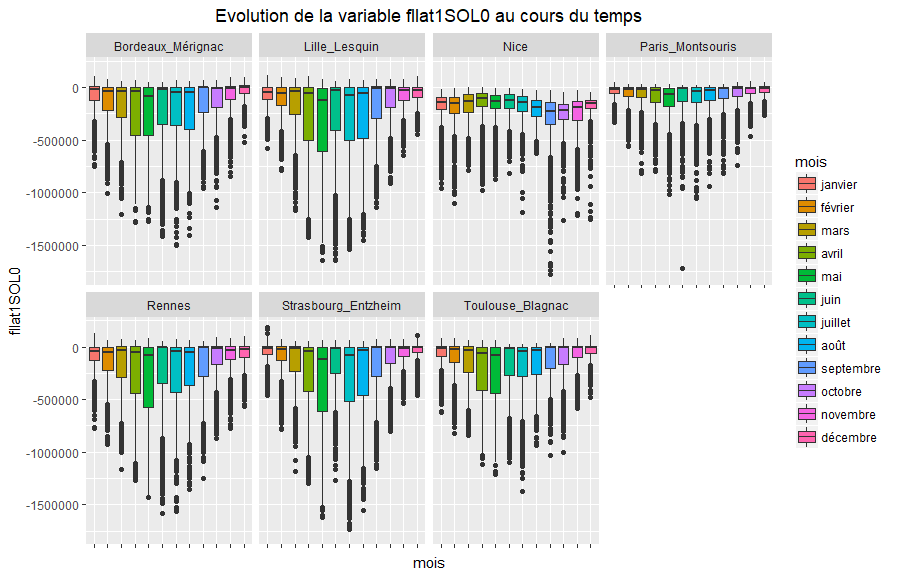
\includegraphics[width=17cm]{Images/fllat.png}
\begin{center}
\captionof{figure}{Exemple du flux de chaleur latente dont le comportement diffère d'une station à une autre}
\label{fig1}
\end{center}
\paragraph{}
Dans la suite, nous verrons que le gros jeu de données ($189281$ lignes) ou les fichiers par stations seront utilisés en fonction de l'algorithme choisi. Une autre option aurait pu être de découper les données par station et par échéance. Cependant en procédant de la sorte, on se retrouverait avec 252 modèles à estimer, et l'on s'exposerait également au risque de sur-apprentissage (\textit{overfitting} en anglais). La dimension des données va également impacter le choix de la méthode d'estimation des paramètres et d'estimation de la performance de l'algorithme : la \textbf{validation croisée}. Nous allons donc effectuer quelques rappels sur ces différents concepts.

\subsection{Notions d'overfitting/underfitting}
\paragraph{}
Comme introduit brièvement un peu plus haut dans ce rapport, l'un des enjeux de ce projet dans le but d'obtenir les meilleurs prédictions possibles, selon le critère du \textbf{RMSE}, sera d'éviter de se retrouver en situation sur-apprentissage ou de sous-apprentissage (respectivement \textit{overfitting} et \textit{underfitting}). En ce sens, on va chercher à construire un estimateur (une fonction) optimal, robuste qui conservera un pouvoir de prédiction de qualité sur un nouvel échantillon. Prenons le dessin suivant qui sera un peu plus parlant.
\paragraph{}
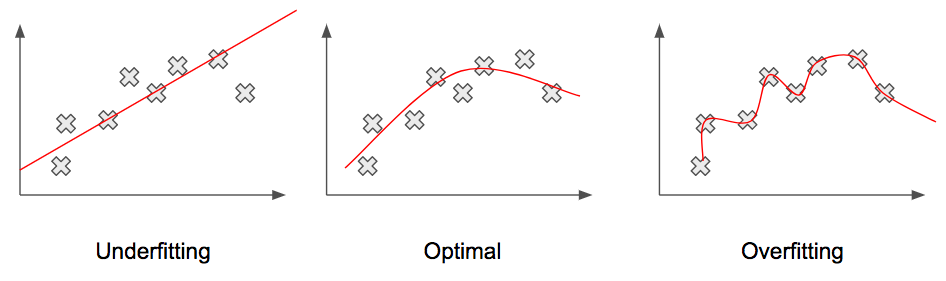
\includegraphics[width=17cm]{Images/overfitting.png}
\begin{center}
\captionof{figure}{Illustration de ces notions à partir d'un exemple simple dans $\mathbb{R}^2$}
\label{fig1}
\end{center}
On s'aperçoit que sur le graphe de gauche, l'estimateur est trop rigide, il ne \og colle \fg{} pas assez aux données. Sur le graphe de droite c'est le contraire, l'estimateur est beaucoup trop sensible aux valeurs, et lorsque les données changeront, les prédictions ne seront donc plus aussi précises. Nous souhaitons donc trouver une fonction ayant une allure similaire à celle du graphe du milieu, qui sera plus \og robuste \fg{} que les deux autres.


Nous verrons dans la suite que pour remédier au problème de l'overfitting, nous pouvons utiliser des formes de \textbf{régularisation}, encore appelées pénalités et qui se traduiront par des contraintes dans le problème d'optimisation d'une certaine \textbf{fonction de perte} que l'on va choisir.\\

Une façon de vérifier que le modèle est robuste peut-être de procéder à de la \textbf{validation croisée}, c'est donc le prochain point que nous allons développer.
 
\subsection{Validation croisée}
\paragraph{}
Comme énoncé précédemment, nous allons utiliser la méthode de la validation croisée à la fois pour contrôler la performance et la robustesse de l'algorithme mis en œuvre, mais également pour calibrer des hyper-paramètres dans le cas de modèles complexes. Nous allons donc dans la suite effectuer quelques rappels théoriques afin de bien comprendre pourquoi nous utilisons cette méthode ainsi qu'une présentation des deux types de validation croisée que nous avons choisi d'utiliser.

\subsubsection{Contexte théorique}
\paragraph{}
Soit $d^{n}_{1}$ l'observation d'un n-échantillon $D^{n}_{1} =$\{$(X_1,Y_1),...,(X_n,Y_n)$\} d'une loi conjointe $P$ sur $\mathcal{X}$ x $\mathcal{Y}$ qui est inconnue. Le premier travail consiste à estimer cette loi $P$ à l'aide des données disponibles, à savoir $d^{n}_{1}$.
\paragraph{}
En théorie, il faudrait minimiser la quantité appelée \textbf{risque} (ou encore \textbf{erreur de généralisation}) d'une règle de prédiction que l'on va noter $f$. Ainsi de façon mathématique, on définit le \textbf{risque} de la manière suivante :
\paragraph{}
$\mathcal{R}_P(f) = \mathbb{E}_{(X,Y)}[l(Y,f(X))]$ avec $l$ que l'on appelle \textbf{fonction de perte} et qui a pour expression :
\begin{itemize}
\item $l(y,y') = |y-y'|^q$ en régression réelle (on prendra souvent la perte \textit{quadratique}, c'est-à-dire lorsque $q=2$)
\item $l(y,y') = \mathds{1}_{y \neq y'} = \frac{|y-y'|}{2} = \frac{|y-y'|^2}{4}$ en discrimination binaire.
\end{itemize}
\paragraph{}
Cependant en pratique, il nous est impossible de calculer le \textbf{risque}. Il faut donc l'estimer et chercher à minimiser cette quantité estimée par la suite. Une première approche naturelle serait d'utiliser le risque empirique, c'est-à-dire d'estimer l'espérance de la fonction de perte par la moyenne empirique de cette même fonction. Le \textbf{risque empirique} d'un algorithme de prédiction $f_{D^{n}_{1}}$ construit sur $D^{n}_{1}$ se note de la façon suivante :
\begin{center}
$\widehat{\mathcal{R}}_n(f_{D^{n}_{1}}) = \frac{1}{n} \sum\limits_{i=1}^n l(Y_i,f_{D^{n}_{1}}(X_i))$
\end{center}

\paragraph{}
Le problème de cet estimateur est l'absence d'indépendance : en effet, pour effectuer nos prédictions on se sert des mêmes données qui ont servi à faire l'algorithme d'apprentissage. En ce sens, notre algorithme risque de trop \og coller \fg{} aux données d'apprentissage, puisqu'il aura acquis l'information à partir de ces données il sera capable de bien prédire la variable réponse, mais risque de ne pas être aussi performant à l'avenir sur un nouveau jeu de données. C'est ce qu'on nous avons défini comme étant l'\textit{overfitting}. C'est donc pour corriger ce problème que nous allons avoir recours à une autre méthode d'estimation du \textbf{risque}, qui est meilleure : la \textbf{validation croisée}.

\subsubsection{La validation croisée Hold-Out}
\paragraph{}
Le concept de base pour la validation croisée \textbf{Hold-Out} consiste à séparer nos données $d^{n}_{1}$ en deux sous-échantillons :
\begin{itemize}
\item $\mathcal{A}$ : l'échantillon d'apprentissage
\item $\mathcal{V}$ : l'échantillon de validation
\end{itemize}
\bigskip
Cela implique d'avoir à la base un jeu de données suffisamment \og grand \fg{} pour pouvoir appliquer une telle méthode, ce qui n'est pas un problème dans notre cas. Comment séparer les données ? En pratique on va diviser notre échantillon en deux parties égales, si l'on dispose d'un échantillon de taille $n$, $\mathcal{A}$ et $\mathcal{V}$ seront donc de taille $\frac{n}{2}$. Si les données sont classées, on procèdera à un tirage aléatoire sans remise de $\frac{n}{2}$ éléments dans $\{1,...,n\}$.
Ensuite on \og nourrit \fg{} notre algorithme à partir des données contenues dans $\mathcal{A}$ et on teste sa performance sur les données de $\mathcal{V}$ : ainsi le problème d'indépendance est réglé. Illustrons cette méthode avec un schéma.\\
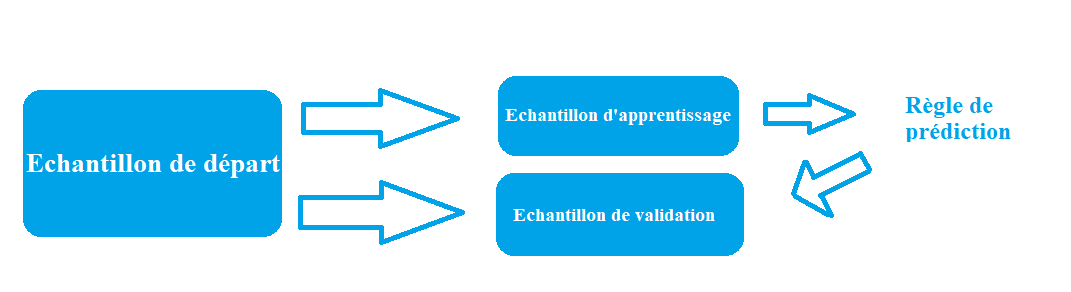
\includegraphics[width=18cm]{Images/hold_out.png}
\begin{center}
\captionof{figure}{Fonctionnement de la validation croisée Hold-Out}
\label{fig1}
\end{center}
\paragraph{}
De façon mathématique, cet estimateur du risque se définit de la façon suivante :
\paragraph{}
$\widehat{\mathcal{R}}(f_{D^{n}_{1}}) = \frac{1}{|\mathcal{V}|} \sum\limits_{i \in \mathcal{V}} l(y_i,f_{d_{\mathcal{A}}}(x_i))$ avec $|\mathcal{V}|$ le cardinal de $\mathcal{V}$ (autrement dit, le nombre de lignes de l'échantillon de validation).
\paragraph{}
Dans le cadre de nos travaux, l'utilisation de cette méthode va nous permettre de gagner du temps si l'on utilise la matrice de travail contenant toutes les stations. La méthode suivante que nous allons présenter prendra plus de temps mais peut apporter plus de stabilité dans les résultats.
\newpage
\subsubsection{La validation croisée K-Fold}
\paragraph{}
La validation croisée \textbf{K-Fold} est une variante de la méthode vue précédemment, qui on le rappelle était adaptée aux jeux de données de taille suffisamment grande. Cependant sur des jeux de données plus petits, comme c'est le cas de nos fichiers par station qui font environ $27000$ lignes chacun,ce type de validation croisée peut également s'avérer efficace. Le fonctionnement de cette méthode itérative est le suivant :
\begin{itemize}
\item On procède à une partition de notre échantillon en $K$ blocs équilibrés : $B_1,...,B_K$ auxquels sont associés des tailles $n_1,...,n_K$. (En pratique on prend $K=10$ quand la taille des données le permet)
\item On note $d_{B_i}=\{(x_j,y_j), j \in B_i\}$ le $i^{eme}$ bloc  de l'échantillon $d^{n}_{1}$. Pour chaque itération $i = 1,...,K$ on laisse de côté les données de $B_i$ pour faire notre apprentissage sur les $K$-1 blocs restants.
\item On teste la performance de notre règle de prédiction sur le bloc $B_i$ pour obtenir une estimation du risque à l'itération $i$ que l'on note : \\ $\widehat{\mathcal{R}}_i = \frac{1}{n_i} \sum\limits_{j \in B_i} l(y_j,f_{d^{n}_{1}} \backslash d_{B_i}(x_j))$
\item Enfin, après avoir procédé à toutes les itérations, on calcule la véritable estimation du risque en faisant la moyenne des risques calculés à chaque itération :\\
$\widehat{\mathcal{R}}(f_{D^{n}_{1}}) = \frac{1}{K} \sum\limits_{i=1}^K \widehat{\mathcal{R}}_i$
\end{itemize}
\paragraph{}
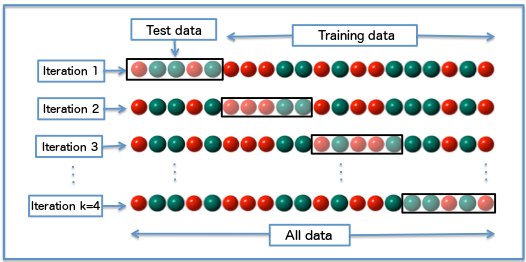
\includegraphics[width=17cm]{Images/k_fold.jpg}
\begin{center}
\captionof{figure}{Exemple de fonctionnement pour K=4}
\label{fig1}
\end{center}
\paragraph{}
Il s'agit désormais d'utiliser la méthode de notre choix dans le but de trouver le meilleur compromis entre précision de l'algorithme et temps de calcul. Le domaine de la \textit{Data Science} fait interagir la théorie mathématique avec la réalisation informatique, il est donc important de prendre en compte ces deux aspects et d'optimiser leur utilisation conjointe au mieux.
\section{Analyse des corrélations entre variables et visualisation}

\newpage
\section{Travail des données}
\paragraph{}
Avant de lancer différents algorithmes sur nos données, il est important de travailler sur des données \og propres \fg{}. Nous allons donc dans la suite détailler les différentes étapes de nettoyage et de tranformation de certaines données.
\subsection{Gestion et remplacement des valeurs manquantes}
\paragraph{}
Une partie clé de cette étude aura été la gestion des valeurs manquantes. En effet, tous les fichiers $train\_H.csv$ $(H=1,..,36)$, en contiennent, ce qui nous a donc amené à nous poser les questions suivantes : faut-il éliminer les lignes contenant des \textit{NA} ? Faut-il remplacer ces valeurs manquantes ? Si oui, pour quelles variables, de quelle façon et à quel coût ? Nous allons détailler l'analyse qui nous a permis de répondre à ces différentes interrogations et de prendre nos décisions.
\paragraph{}
Premièrement nous avons regardé s'il était possible de remplacer les valeurs sur toutes les variables qui en contiennent dans nos données. Toutes les variables numériques (i.e qui ne sont pas des facteurs) en contiennent. Le graphe suivant nous montre l'erreur moyenne pour chaque variable après des tentatives d'imputation par \textbf{moyenne}, \textbf{médiane}, \textbf{10-NN}, \textbf{Random Forest} et \textbf{décalage temporel} (par exemple s'il manque une valeur pour la variable \textit{ux1H10} à Bordeaux le 20/06/2015 à l'échéance 1, on va remplacer cette valeur par celle de la même date et de la même station à l'échéance 2).

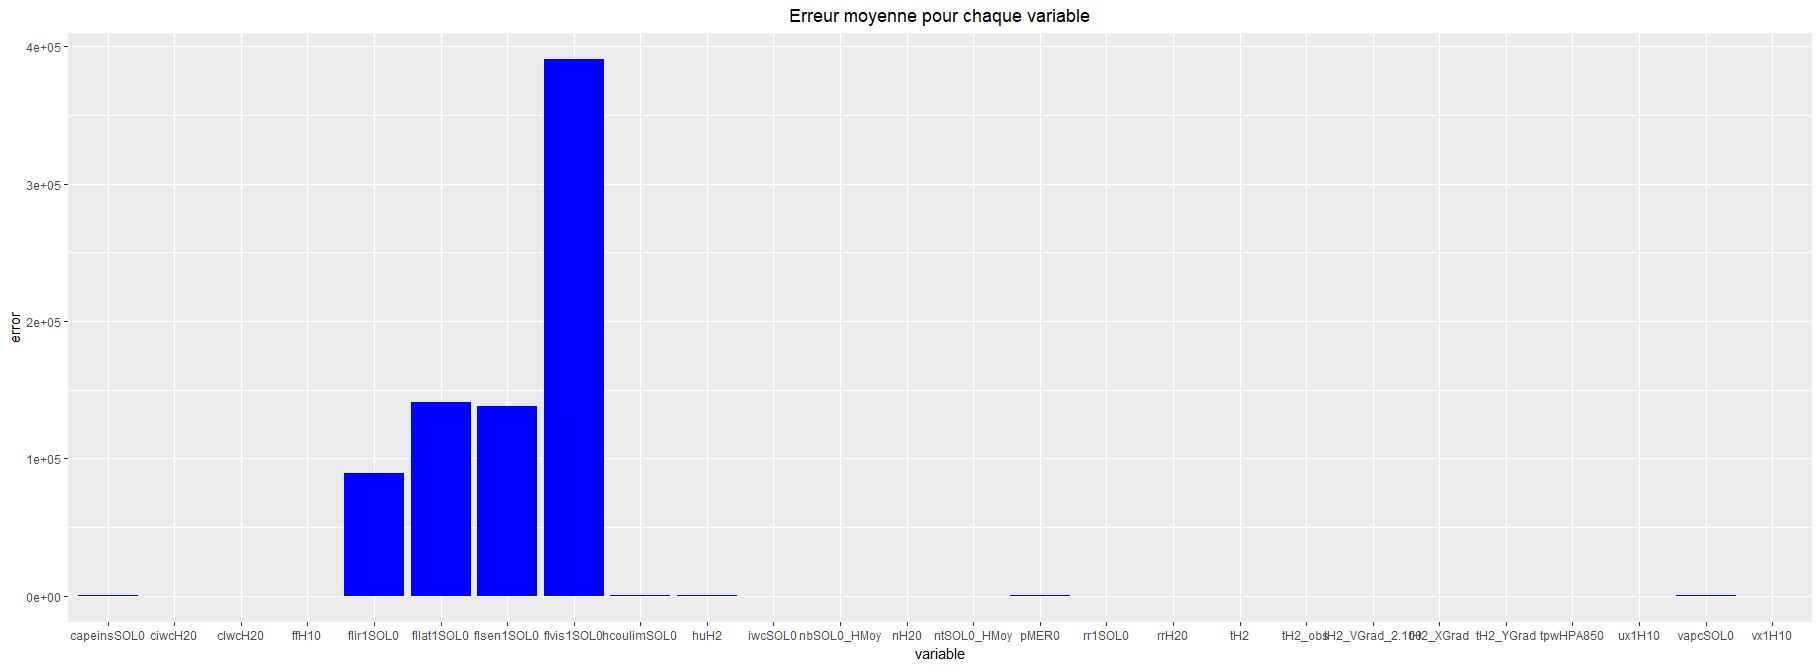
\includegraphics[width=17cm]{Images/na_error.png}
\begin{center}
\captionof{figure}{L'imputation de certaines variables semble problématique}
\label{fig1}
\end{center}
\paragraph{}
Clairement, ce graphique fait ressortir un problème pour les variables \textbf{flir1SOL0}, \textbf{fllat1SOL0}, \textbf{flsen1SOL0}, \textbf{flvis1SOL0} et dans une moindre mesure pour les variables \textbf{hcoulimSOL0} et \textbf{capeinsSOL0}. Nous avons donc décider de ne pas remplacer les valeurs manquantes pour ces variables, puisque les remplacer pourrait potentiellement être pire pour la qualité de notre analyse.


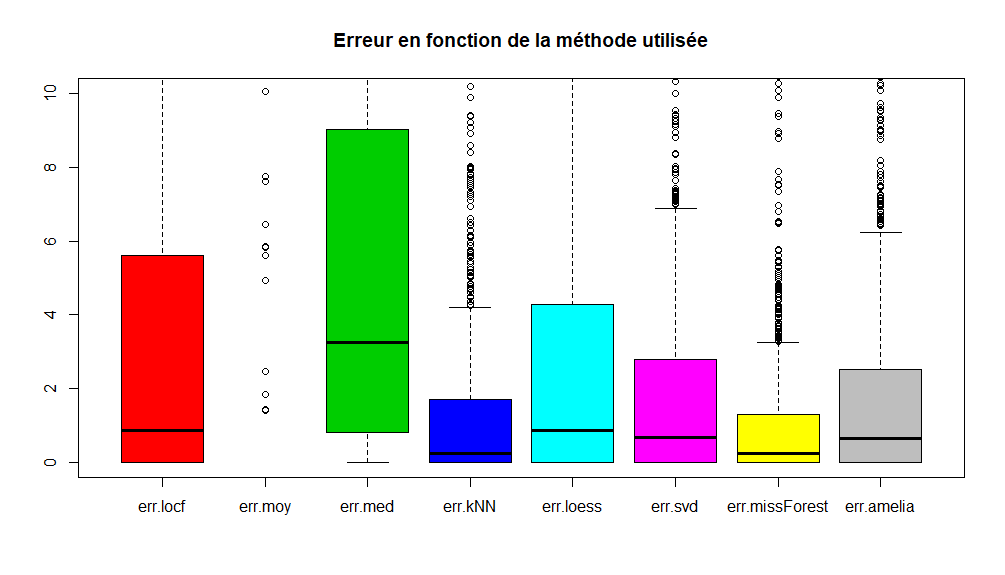
\includegraphics[width=17cm]{Images/err_imp.png}
\begin{center}
\captionof{figure}{Taux d'erreur des méthodes d'imputation testées}
\label{fig1}
\end{center}

\subsection{Transformation de la date}

\section{Choix et application d'algorithmes d'apprentissage supervisé}

\subsection{Premiers algorithmes : la régression linéaire et ses variantes}

\subsection{Forêt aléatoire : l'algorithme Random Forest}

\subsection{Gradient Boosting : l'algorithme XGBoost}

\subsection{Deep Learning : l'utilisation des réseaux de neurones}
\paragraph{}
Le Deep Learning permet de résoudre différents problèmes que nous pouvons rencontrer avec les réseaux de neurones comme la stabilité. Aujourd'hui il est souvent utilisé pour des problèmes divers avec des résultats parfois remarquable comme nous pouvons le voir avec le site de traduction DeepL, le plus abouti aujourd'hui pour le grand public ou encore pour des outils d'analyse des émotions par un visage photographié ou filmé.

Le principe de base du modèle (montré dans l'image ci-dessous) est le neurone, un modèle d'inspiration biologique du neurone humain. Chez l'homme, les différents niveaux de puissance des signaux de sortie des neurones circulent le long des jonctions synaptiques et sont ensuite agrégés en entrée pour l'activation d'un neurone connecté. On appelle ce modèle le modèle \textbf{perceptron}.

Dans le modèle la combinaison pondérée, La fonction f représente la fonction d'activation non linéaire utilisée dans tout le réseau et le biais $\beta_{0} $ représente le seuil d'activation du neurone. :
\begin{center}
$y_{i}=f(\beta_{0} + \sum\limits_{j} \beta_{j}x_{i,j}) + \varepsilon_{i}$
\end{center}


\section{Bilan}

\section{Bibliographie et sources}

\begin{flushleft}
- \textbf{WikiStat}, \href{https://www.math.univ-toulouse.fr/~besse/Wikistat/pdf/st-scenar-app-idm.pdf}{\textit{\textcolor{blue}{Scénario: Imputation de données manquantes}}}\\
\medskip
\end{flushleft}

\end{document}
